\section{Datasets used}
The $h \rightarrow aa \rightarrow 2b2\tau$ analysis (CMS CADI line HIG-22-007) is based on proton-proton collision data at a center-of-mass energy of 13 TeV collected in full Run-2 (2016-18) with the CMS detector. The data analyzed corresponds to a total integrated luminosity of 138 fb$^{-1}$ (36.33 fb$^{-1}$ for 2016, 41.53 fb$^{-1}$ for 2017, and 59.74 fb$^{-1}$ for 2018) \cite{CMS-LUM-17-001} \cite{CMS-LUM-17-004} \cite{CMS-LUM-18-002}. 

Data collected with the single muon trigger is used for the $\mu\tau_{h}$ channel. For the $e\tau_{h}$ channel, data collected with the single electron trigger is used; and for the $e\mu$ channel, data collected with the electron $+$ muon trigger is used. A more in-depth discussion of the triggers used follows in a later section.

A full list of samples used can be found in the full documentation \cite{CMS-HIG-22-007} \cite{CMS-PAS-HIG-22-007}.

\section{Monte Carlo samples}
Modeling and computing observables originating from arbitrary physics processes at the tree level and at next-to-leading order (NLO) is performed by Monte Carlo (MC) event generators, such as Powheg and MadGraph5\_amC\@NLO \cite{Alwall_2014} \cite{Frederix_2018}. The information generated, e.g. the computation of the differential cross sections and kinematics of the final state particles, is saved in a compressed file and used to generate MC samples that are used in physics analyses. The samples are digitized using GEANT4 \cite{agostinelli_geant4simulation_2003}, a platform used at the LHC and other facilities to comprehensively simulate the passage of particles through matter. The digitized samples are passed through the same detector reconstruction as real data events collected in the detector.

The samples for modeling the signal ($h \rightarrow aa \rightarrow 2b2\tau$ and $h\rightarrow a_1 a_2$) in the 2HDM+S and TRSM are generated at tree-level, for a range of masses of the light neutral scalar $a$. For $h \rightarrow aa$, the mass hypotheses for the $a$ range from $m_a = (12 \,\text{GeV}, 62.5 \,\text{GeV})$. For $h \rightarrow a_1 a_2$, the mass hypotheses for the two light scalars span combinations of $m_{a1}$, $m_{a2}$ ranging from $(12 \,\text{GeV}, 62.5 \,\text{GeV})$ for the two scalars.


\section{Embedded samples}
\label{sec:embedded-samples}
An embedding technique is used to estimate background from the Standard Model $Z$ boson decaying to $\tau\tau$, from data with minimal simulation input \cite{CMS-TAU-18-001}. In data events containing $Z \rightarrow \mu\mu$ decays, all energy deposits of the recorded muons are removed from the event, and replaced with simulated tau leptons with the same kinematic properties as the removed muons. This results in a hybrid data format containing information from both observed and simulated events, as illustrated in Fig. \ref{fig:embedded-schematic} \cite{CMS-TAU-18-001}. The advantage of the Embedded samples is that the portions of the event that are difficult to model and describe (e.g. the underlying event or production of additional jets) are directly taken from data. 

% TODO: add text

\begin{figure}[h]
    \centering
    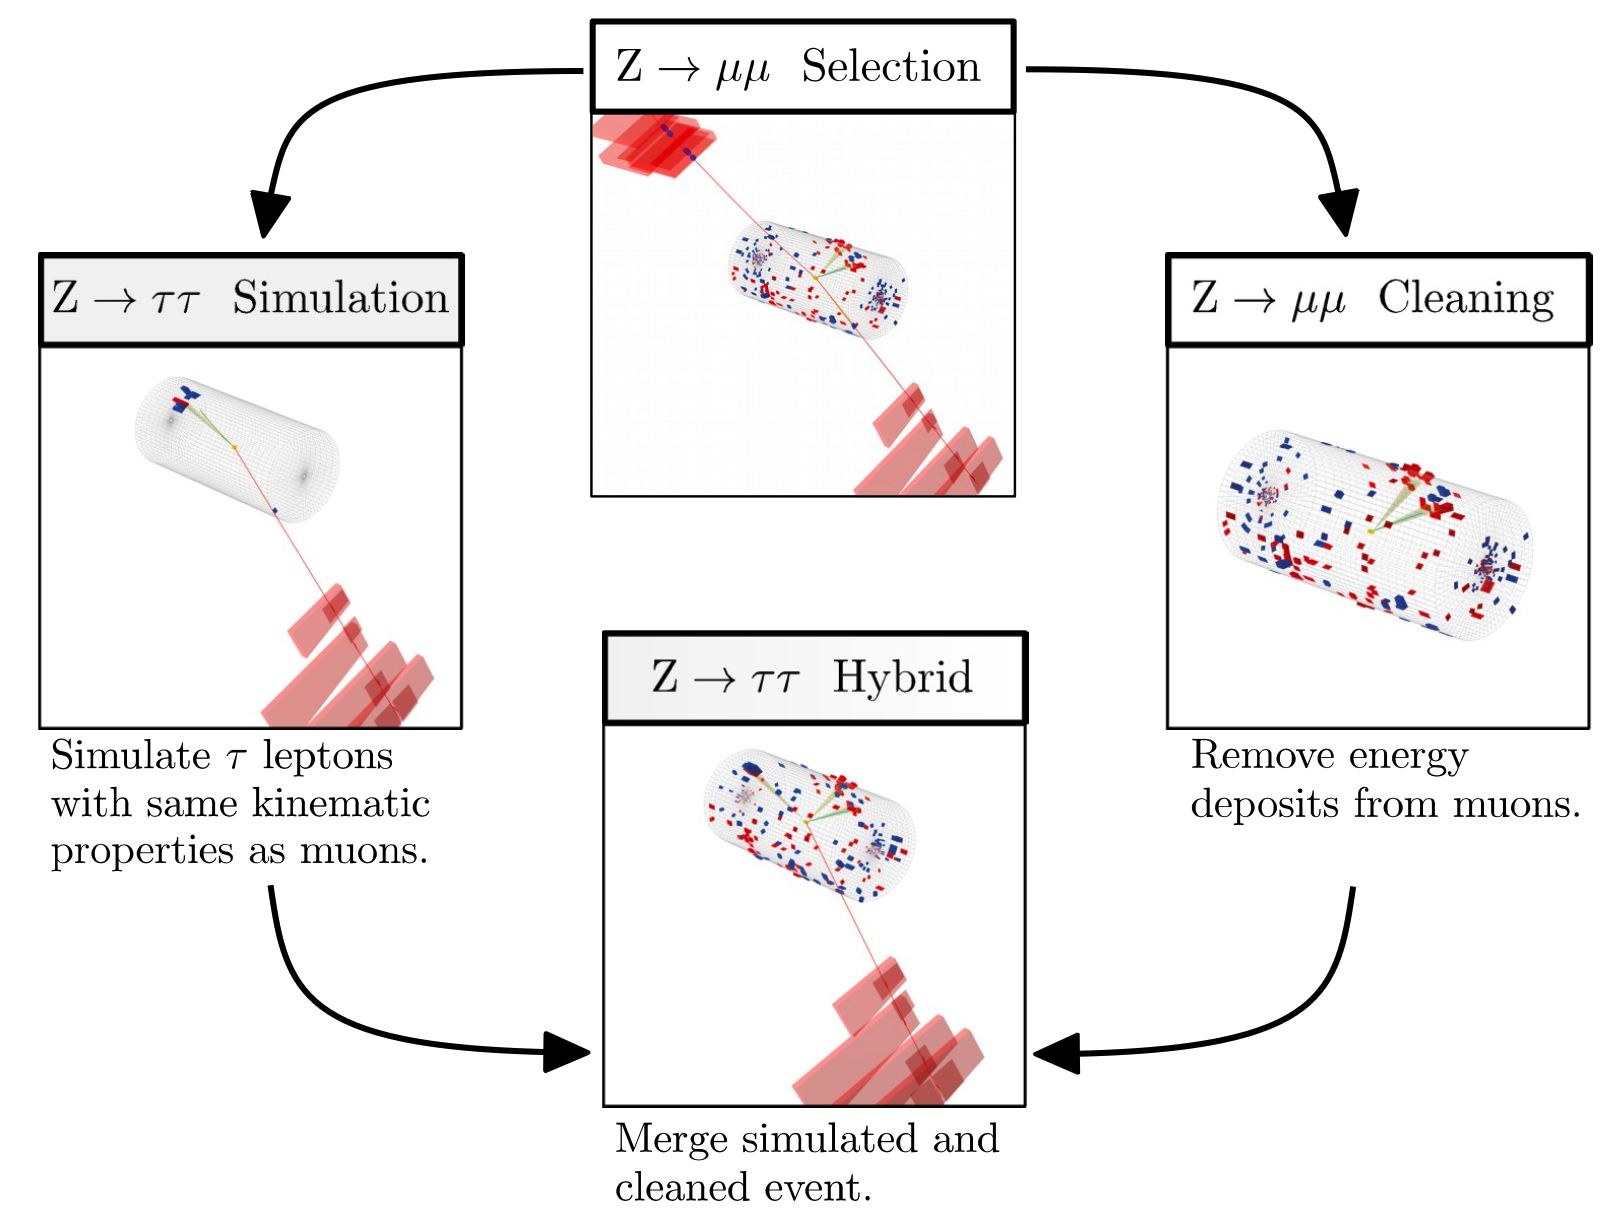
\includegraphics[width=15cm]{figures/ch-4-datasets-monte-carlo/embedded_schematic}
    \caption[Schematic view of the four main steps of the embedding technique for $\tau$ leptons.]{Schematic view of the four main steps of the embedding technique for $\tau$ leptons, as described in Section \ref{sec:embedded-samples} \cite{CMS-TAU-18-001}. A $Z \rightarrow \mu\mu$ event is selected in data (\textit{$Z\rightarrow \mu\mu$ selection}), all of the energy deposits associated with the muons are removed (\textit{$Z \rightarrow \mu\mu$ cleaning}), and two $\tau$ leptons and their decays are simulated in an empty detector (\textit{$Z \rightarrow \tau\tau$ simulation}). Lastly, all energy deposits of the simulated $\tau$ decays are combined with the data event (\textit{$Z \rightarrow \tau\tau$ hybrid}).} 
    \label{fig:embedded-schematic}
\end{figure}
